\subsubsection{الگوی \lr{Layered}}
\label{archLayerSec}
\begin{RTL}
الگوی لایه‌ای \cite{ref4} دامنه‌های سیستم را بر اساس سطوح انتزاعی
مختلف به صورت سلسله‌مراتبی
سازمان‌دهی می‌کند. مفاهیم انتزاعی‌تر در یک دامنه با استفاده
از مفاهیم ملموس‌تر در دامنه‌های دیگر پیاده‌سازی می‌شوند.
این ساختار به متخصصان اجازه می‌دهد تا به طور موثر در زمینه تخصصی
خود کار کنند بدون اینکه نیاز به درک تمامی جزئیات زیرین
داشته باشند. به همین ترتیب، در توسعه نرم‌افزار،
دامنه‌های انتزاعی با استفاده از دامنه‌های ملموس‌تر پیاده‌سازی
می‌شوند که این امر موجب سازمان‌دهی و قابلیت تطبیق‌پذیری بیشتر بین
پلتفرم‌های مختلف می‌شود.
\end{RTL}
\begin{figure}[h!]
\centering
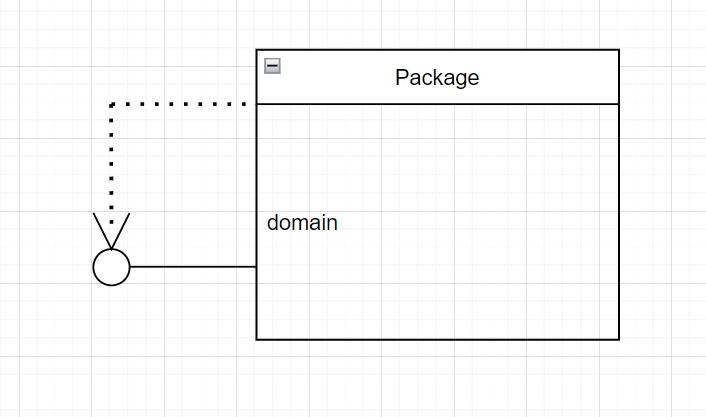
\includegraphics[scale=0.5]{images/first/layer.png}
\caption{ساختار الگوی \lr{Layered}}
\end{figure}